\chapter{RISC-V}
\label{cha:riscv}

RISC-V is an open-source, modular Instruction Set Architecture (ISA) developed by
the University of California, Berkeley\cite{riscv}. Unlike proprietary ISAs such
as ARM and x86, RISC-V is designed to be flexible and extensible, enabling
researchers, developers, and companies to build custom processors without
licensing fees. This chapter provides a detailed background on the RISC-V architecture,
which forms the foundation for the security enhancements discussed in this
thesis.

The core design philosophy behind RISC-V emphasizes simplicity, modularity, and
extensibility. Its open nature and clean-slate design approach make it a preferred
platform for developing secure and innovative hardware solutions, as
demonstrated in this project.

\section{RISC-V Instruction Set Architecture Overview}
\label{sec:riscv_isa}

The RISC-V ISA is structured around a minimal base integer ISA, which is
mandatory for all implementations, supplemented by optional extensions. This
base is designed with simplicity in mind, providing enough instructions for essential
software tools like compilers and operating systems while allowing for extensive
customization and specialization through additional extensions.

There are four main base ISAs within the RISC-V family: RV32I, RV64I, RV32E, and
RV64E, each differing primarily in the width of integer registers (32 or 64 bits)
and the number of available registers. These variations support different use cases,
from small microcontrollers (RV32E and RV64E) to larger systems (RV64I).

To accommodate customization, RISC-V divides instruction encoding space into three
categories: standard (defined by RISC-V International), reserved (for future use),
and custom (for vendor-specific extensions). This segmentation supports the creation
of specialized ISAs without conflicting with the core architecture.

Overall, the RISC-V ISA is designed to support energy-efficient and specialized
computing, prioritizing flexibility and modularity over legacy compatibility.

\section{RISC-V Base Instruction Formats}
\label{sec:riscv_bif}

The base RV32I ISA uses four main instruction formats: \texttt{R}, \texttt{I}, \texttt{S},
and \texttt{U}, all fixed at 32 bits and aligned to a four-byte boundary in memory
(shown in Figure \ref{fig:instrformats}).

Additionally, RV32I includes formats \texttt{B} and \texttt{J} (shown in Figure \ref{fig:extrainstrformats}),
which vary in immediate encoding to optimize hardware design. The immediate
structure across formats is designed to minimize hardware complexity and overlap,
focusing on efficiency for both compilation and runtime execution. Sign-extension
and fixed bit positioning help reduce hardware costs and reducing complexity in
simple implementations.

\begin{figure}[htbp]
  \centering
  \def\stackalignment{r}\stackunder{ 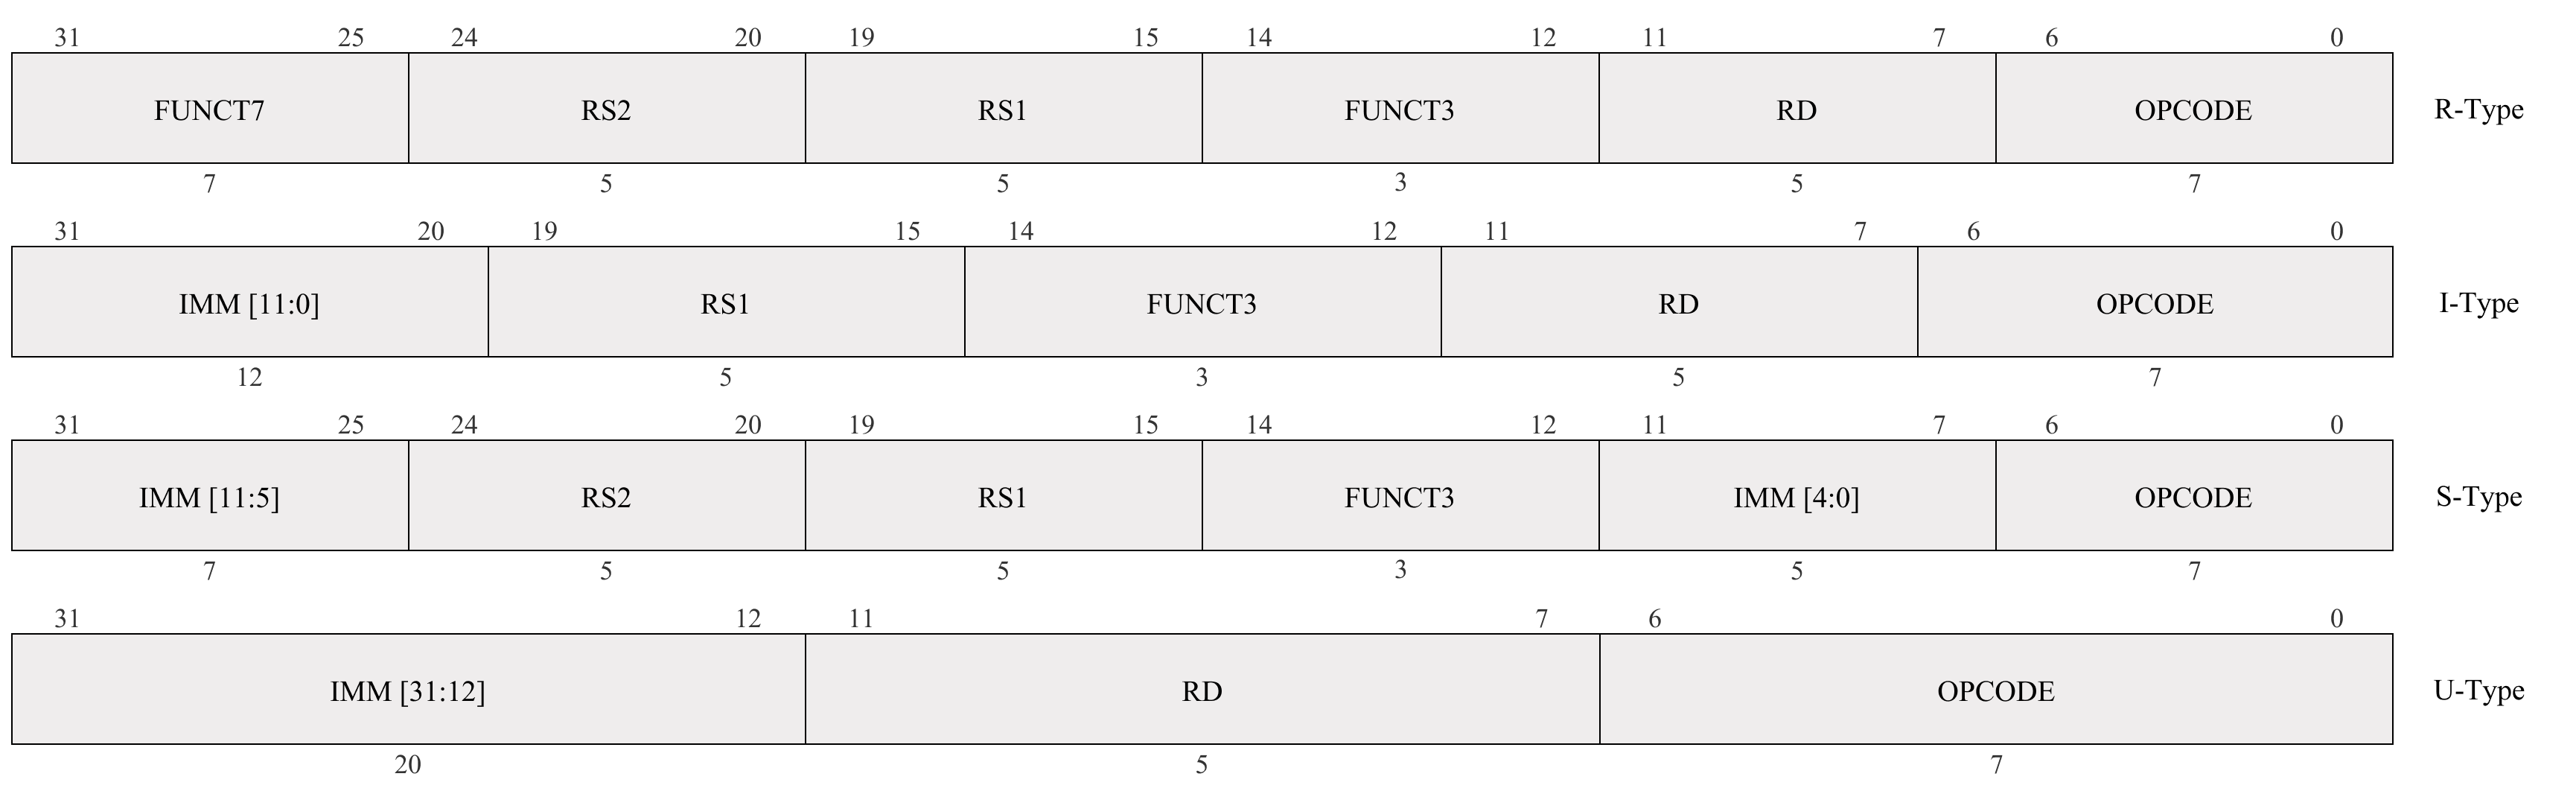
\includegraphics[width=.9\linewidth]{images/instrformats.png}}
  {\scriptsize }
  \caption{RISC-V Base Instruction Formats}
  \label{fig:instrformats}
\end{figure}

\begin{figure}[htbp]
  \centering
  \def\stackalignment{r}\stackunder{ 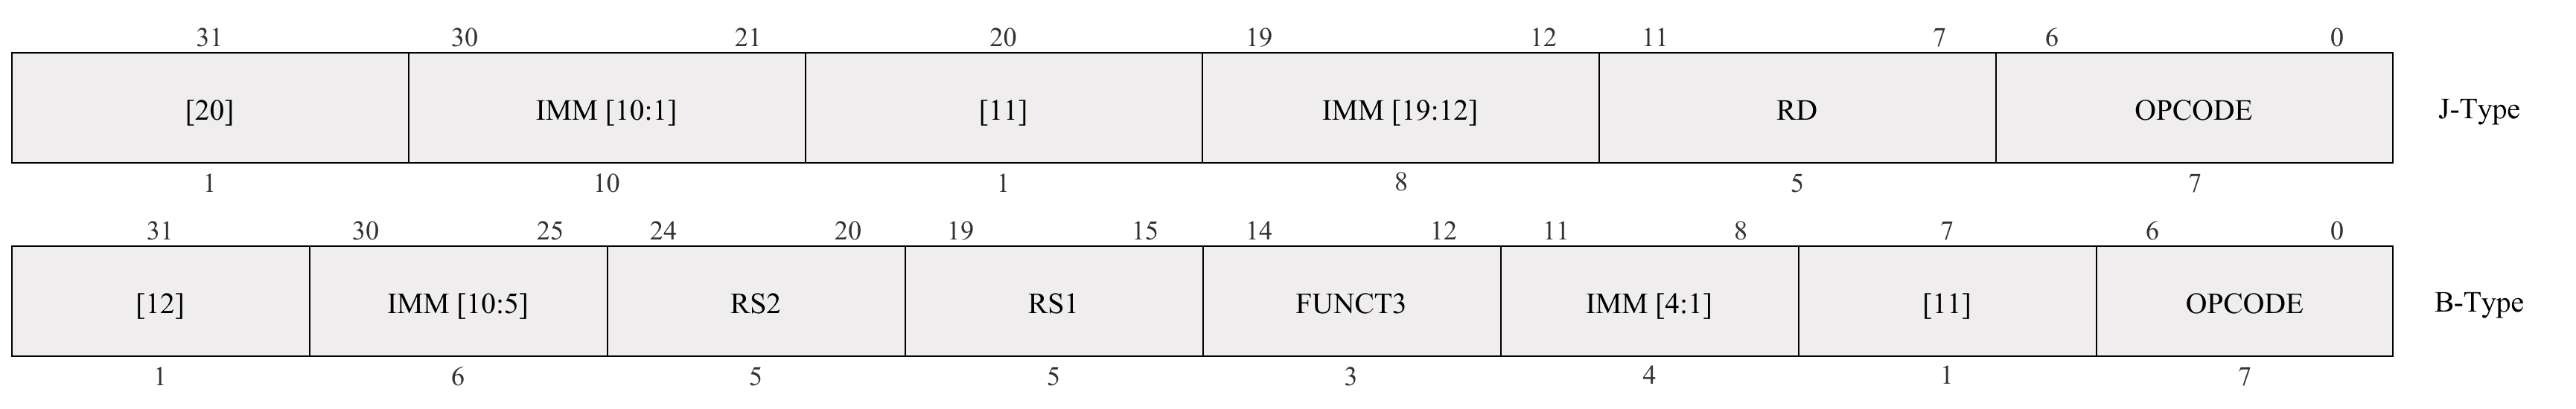
\includegraphics[width=.9\linewidth]{images/extrainstrformats.png} } %
  {\scriptsize }
  \caption{RISC-V Extra Instruction Formats}
  \label{fig:extrainstrformats}
\end{figure}

\section{RISC-V Extensions}
\label{sec:riscv_extensions}

RISC-V’s standard extensions are officially supported and maintained by RISC-V International.
They add functionality to the base ISA while ensuring compatibility across
different implementations. These extensions are designed to enhance performance,
reduce power consumption, or expand the processor's capability to handle specific
tasks efficiently (standard extensions can be seen in Table \ref{tab:extensions}).

Standard extensions can be used together to obtain the needed capabilities for each
specific situation. Moreover, RISC-V’s open architecture allows for the creation
of custom extensions, enabling developers to implement specialized instructions
for domain-specific optimizations. However, while these custom extensions
provide powerful optimizations, they are not standardized, so compatibility
across different implementations is not guaranteed.

\begin{table}
  \centering
  \begin{tabular}{|c|c|}
    \hline
    \textbf{Extension} & \textbf{Description}                \\
    \hline
    A                  & Atomic instructions                 \\
    \hline
    B                  & Bit manipulation                    \\
    \hline
    C                  & Compressed instructions             \\
    \hline
    D                  & Double-precision floating-point     \\
    \hline
    F                  & Single-precision floating-point     \\
    \hline
    G                  & Shorthand for IMAFD extensions      \\
    \hline
    H                  & Hypervisor extension                \\
    \hline
    J                  & Dynamically translated languages    \\
    \hline
    L                  & Decimal floating-point              \\
    \hline
    M                  & Integer multiplication and division \\
    \hline
    N                  & User-level interrupts               \\
    \hline
    P                  & Packed-SIMD instructions            \\
    \hline
    Q                  & Quad-precision floating-point       \\
    \hline
    S                  & Supervisor mode                     \\
    \hline
    T                  & Transactional memory                \\
    \hline
    V                  & Vector operations                   \\
    \hline
  \end{tabular}
  \caption{RISC-V standard extensions}
  \label{tab:extensions}
\end{table}

\section{RISC-V Exceptions, Traps and Interrupts}
\label{sec:riscv_eti}

\lipsum[1]

\section{RISC-V RVWMO Memory Consistency Model}
\label{sec:riscv_rvwmo}

\lipsum[1]

\section{RISC-V Privilege Levels}
\label{sec:riscv_privileges}

RISC-V defines multiple privilege levels to manage access to system resources
and control execution modes. These privilege levels are designed to provide a secure
and efficient framework for managing different software components, such as
operating systems, hypervisors, and user applications.

As it's possible to see in Table \ref{tab:priv} RISC-v implements three
different privilege levels with the following characteristics:

\begin{itemize}
  \item Machine Mode (M-mode): Machine mode is the most privileged and
    fundamental level in the RISC-V architecture. It is the only required privilege
    level in all RISC-V implementations and provides complete access to hardware
    resources and system configurations. It is responsible for configuring the
    hardware, setting up system resources, and initializing other privilege
    levels. Furthermore, Trap Handling is performed by M-mode has;

  \item Supervisor Mode (S-mode): Supervisor mode is an optional privilege level
    designed for running operating systems or hypervisors. It offers more privileges
    than U-mode but less than M-mode. S-mode enables an operating system to
    manage resources and control hardware with enough authority while ensuring
    that user applications cannot access or alter critical system configurations;

  \item User Mode (U-mode): User mode is the least privileged level and is
    designed for running user-level applications. It restricts access to critical
    system resources, ensuring that any malicious or faulty application cannot
    compromise the overall system. U-mode’s restricted environment makes it ideal
    for running user applications securely, providing a balance between
    performance and protection.
\end{itemize}

\begin{table}
  \centering
  \begin{tabular}{|c|c|c|c|}
    \hline
    \textbf{Level} & \textbf{Encoding} & \textbf{Name}    & \textbf{Abbreviation} \\
    \hline
    0              & 00                & User/Application & U                     \\
    \hline
    1              & 01                & Supervisor       & S                     \\
    \hline
    2              & 10                & Reserved         &                       \\
    \hline
    3              & 11                & Machine          & M                     \\
    \hline
  \end{tabular}
  \caption{RISC-V privilege levels}
  \label{tab:priv}
\end{table}

\section{RISC-V General Purpose Registers}
\label{sec:riscv_reg}

\lipsum[1]

\section{RISC-V Control and Status Registers (CSRs)}
\label{sec:riscv_csrs}

\lipsum[1]

\section{RISC-V Physical Memory Protection (PMP)}
\label{sec:riscv_pmp}

\lipsum[1]

\section{RISC-V Toolchain}
\label{sec:riscv_toolchain}

\lipsum[1]

% ## 2.2 Architecture Overview

% The RISC-V architecture follows the Reduced Instruction Set Computer (RISC) principles, focusing on a minimalistic set of instructions to ensure simplicity and efficiency. The basic ISA consists of the following components:

% - **Base ISA (RV32I/RV64I)**: The core instruction set provides the essential operations, including arithmetic, logic, control, and memory access instructions. The ISA supports both 32-bit (RV32) and 64-bit (RV64) implementations, with each offering compatibility and scalability across different application domains.

% - **Modularity**: RISC-V's modular approach allows additional features and capabilities through optional extensions, making it a highly customizable platform. This flexibility enables targeted enhancements, such as security features and performance optimizations tailored to specific use cases.

% ## 2.3 Base Instruction Set and Modularity

% The base instruction set (RV32I) comprises a limited but sufficient set of instructions, ensuring the simplicity and efficiency of hardware implementations. RISC-V further extends this base with several optional extensions, enabling diverse functionality:

% - **Instruction Set Extensions**:
%   - **M Extension**: Adds support for integer multiplication and division.
%   - **A Extension**: Provides atomic operations essential for building multithreaded applications.
%   - **F and D Extensions**: Introduce support for single-precision (F) and double-precision (D) floating-point operations, respectively, critical for numerical and scientific computations.
%   - **C Extension**: Implements compressed instructions to reduce code size, particularly beneficial for embedded systems and memory-constrained environments.

% These extensions allow RISC-V to be adapted for various applications, from microcontrollers and embedded systems to high-performance computing platforms.

% ## 2.4 Registers and Control and Status Registers (CSRs)

% RISC-V defines several key register types:

% - **General-Purpose Registers (GPRs)**: The base ISA defines 32 general-purpose registers (`x0` to `x31`) for arithmetic, logic, and memory operations. Register `x0` is hardwired to zero, simplifying certain operations.

% - **Control and Status Registers (CSRs)**: CSRs are used to manage and control various aspects of the processor, such as privilege levels, interrupt handling, and performance monitoring. These registers play a crucial role in configuring and managing security features like Physical Memory Protection (PMP) and the shadow stack, which are elaborated upon later in this thesis.

% ## 2.5 Privilege Levels

% RISC-V supports multiple privilege levels to isolate and manage system resources:

% - **Machine Mode (M-mode)**: The highest privilege level, responsible for low-level hardware control. In M-mode, the processor can access all system resources, making it crucial for boot processes and managing secure functions.

% - **Supervisor Mode (S-mode)**: S-mode is used by operating systems to manage hardware resources and provide services to user applications while maintaining isolation from M-mode.

% - **User Mode (U-mode)**: The least privileged level, primarily for user applications. U-mode cannot directly access critical system resources, enhancing security by isolating user programs from the core hardware.

% By segregating these privilege levels, RISC-V can effectively manage and secure access to critical system components, which is vital in implementing robust security mechanisms.

% ## 2.6 Interrupts and Traps

% RISC-V handles interrupts and traps through a well-defined and flexible mechanism:

% - **Interrupts**: Events that temporarily halt the processor's current operations to execute an Interrupt Service Routine (ISR). Interrupts can be internal (e.g., timer) or external (e.g., hardware device signals).

% - **Traps**: These occur when an exception is detected, such as illegal instruction execution or access to unauthorized memory regions. Traps are crucial for enforcing control and security policies.

% The architecture includes a **Trap-Vector Base Address Register (TVBR)** that helps manage and direct interrupts and traps efficiently. The integration and customization of this mechanism form a critical part of the security enhancements developed in this project.

% ## 2.7 Physical Memory Protection (PMP)

% Physical Memory Protection (PMP) is a hardware feature in RISC-V that allows fine-grained control over memory access permissions. PMP is critical for enforcing memory isolation, which is essential in building secure systems. Key aspects include:

% - **Configuring Memory Regions**: PMP enables the definition of memory regions with specific access permissions (e.g., read, write, execute). This helps in preventing unauthorized access and controlling the execution of code.

% - **Runtime Configuration**: PMP regions can be dynamically adjusted during runtime, offering flexibility for embedded systems and environments where security policies may need to adapt based on operational states.

% In this project, PMP is leveraged to secure the memory layout, isolating sensitive code regions and data structures to prevent unauthorized access and code injection attacks.

% ## 2.8 Toolchain and Development Environment

% The RISC-V ecosystem is supported by a rich set of development tools essential for software and hardware development. The primary components include:

% - **Compiler (GCC)**: The RISC-V GCC compiler is used to generate machine code from high-level languages like C/C++. It supports extensions and customizations, allowing the integration of specific security mechanisms implemented in this project.

% - **Assembler and Linker**: These tools translate assembly language code into machine code and resolve addresses during the linking process, enabling the creation of executable files tailored for RISC-V processors.

% - **Debugger (GDB)**: GDB for RISC-V offers debugging capabilities that are essential for testing and validating code, particularly when implementing and verifying new architectural features.

% - **Simulators (Spike and QEMU)**: These tools emulate RISC-V processors, providing a software-based platform for development and testing. Simulators are crucial for experimenting with architectural changes without needing physical hardware, allowing rapid prototyping and validation of security features before deployment.

% ## 2.9 Summary

% This chapter has outlined the fundamental aspects of the RISC-V architecture, providing the necessary context for understanding the modifications and security mechanisms introduced in this thesis. By detailing the base ISA, extensions, privilege levels, PMP, and the development toolchain, we establish a comprehensive foundation for the subsequent chapters, where these elements are integrated and extended to enhance the security capabilities of the RISC-V platform.

% ---

% This draft provides an in-depth explanation of RISC-V's architecture, preparing the reader for the more technical details and project-specific information that follows in your thesis. Let me know if you'd like any modifications or further details on a specific section!